%% ****** Start of file template.aps ****** %
%%
%%
%%   This file is part of the APS files in the REVTeX 4 distribution.
%%   Version 4.0 of REVTeX, August 2001
%%
%%
%%   Copyright (c) 2001 The American Physical Society.
%%
%%   See the REVTeX 4 README file for restrictions and more information.
%%
%
% This is a template for producing manuscripts for use with REVTEX 4.0
% Copy this file to another name and then work on that file.
% That way, you always have this original template file to use.
%
% Group addresses by affiliation; use superscriptaddress for long
% author lists, or if there are many overlapping affiliations.
% For Phys. Rev. appearance, change preprint to twocolumn.
% Choose pra, prb, prc, prd, pre, prl, prstab, or rmp for journal
%  Add 'draft' option to mark overfull boxes with black boxes
%  Add 'showpacs' option to make PACS codes appear
%  Add 'showkeys' option to make keywords appear
\documentclass{revtex4}
%\documentclass[aps,prl,preprint,superscriptaddress]{revtex4}
%\documentclass[aps,prl,twocolumn,groupedaddress]{revtex4}
\usepackage[dvipdf]{graphicx}
%\usepackage{dcolumn}

% You should use BibTeX and apsrev.bst for references
% Choosing a journal automatically selects the correct APS
% BibTeX style file (bst file), so only uncomment the line
% below if necessary.
%\bibliographystyle{apsrev}

\begin{document}

% Use the \preprint command to place your local institutional report
% number in the upper righthand corner of the title page in preprint mode.
% Multiple \preprint commands are allowed.
% Use the 'preprintnumbers' class option to override journal defaults
% to display numbers if necessary
%\preprint{}

%Title of paper
\title{Isuscipit Lobortis Nisl ut Aliquip ex Ea Commodo}

% repeat the \author .. \affiliation  etc. as needed
% \email, \thanks, \homepage, \altaffiliation all apply to the current
% author. Explanatory text should go in the []'s, actual e-mail
% address or url should go in the {}'s for \email and \homepage.
% Please use the appropriate macro foreach each type of information

% \affiliation command applies to all authors since the last
% \affiliation command. The \affiliation command should follow the
% other information
% \affiliation can be followed by \email, \homepage, \thanks as well.
\author{Jason P. Longacre}
%\homepage[]{Your web page}
%\thanks{}
%\altaffiliation{}
\affiliation{Physics 2501, University of Connecticut}
%\author{R.T. Jones}
%\affiliation{University of Connecticut}

%Collaboration name if desired (requires use of superscriptaddress
%option in \documentclass). \noaffiliation is required (may also be
%used with the \author command).
%\collaboration can be followed by \email, \homepage, \thanks as well.
%\collaboration{}
%\noaffiliation

\date{\today}

\begin{abstract}
Lorem ipsum dolor sit amet, consectetuer adipiscing elit, sed diam
nonummy nibh euismod tincidunt ut laoreet dolore magna aliquam erat
volutpat. Ut wisi enim ad minim veniam, quis nostrud exerci tation
ullamcorper suscipit lobortis nisl ut aliquip ex ea commodo consequat.
Duis autem vel eum iriure dolor in hendrerit in vulputate velit esse
molestie consequat, vel illum dolore eu feugiat nulla facilisis at
vero eros et accumsan et iusto odio dignissim qui blandit praesent
luptatum zzril delenit augue duis dolore te feugait nulla facilisi.
\end{abstract}

% insert suggested PACS numbers in braces on next line
%\pacs{}
% insert suggested keywords - APS authors don't need to do this
%\keywords{}

\setlength{\topmargin}{0in}

%\maketitle must follow title, authors, abstract, \pacs, and \keywords
\maketitle

% body of paper here - Use proper section commands
% References should be done using the \cite, \ref, and \label commands

%% The normal text is displayed in two-column format, but special
%% sections spanning both columns can be inserted within the page
%% format so that long equations can be displayed. Use
%% sparingly.
%%\begin{widetext}
%% put long equation here
%%\end{widetext}
%
%% figures should be put into the text as floats.
%% Use the graphics or graphicx packages (distributed with LaTeX2e)
%% and the \includegraphics macro defined in those packages.
%% See the LaTeX Graphics Companion by Michel Goosens, Sebastian Rahtz,
%% and Frank Mittelbach for instance.
%%
%% Here is an example of the general form of a figure:
%% Fill in the caption in the braces of the \caption{} command. Put the label
%% that you will use with \ref{} command in the braces of the \label{} command.
%% Use the figure* environment if the figure should span across the
%% entire page. There is no need to do explicit centering.
%
%%\begin{turnpage}
%% Surround figure environment with turnpage environment for landscape
%% figure
%% \begin{turnpage}
%% \begin{figure}
%% \includegraphics{}%
%% \caption{\label{}}
%% \end{figure}
%% \end{turnpage}
%
%% tables should appear as floats within the text
%%
%% Here is an example of the general form of a table:
%% Fill in the caption in the braces of the \caption{} command. Put the label
%% that you will use with \ref{} command in the braces of the \label{} command.
%% Insert the column specifiers (l, r, c, d, etc.) in the empty braces of the
%% \begin{tabular}{} command.
%% The ruledtabular enviroment adds doubled rules to table and sets a
%% reasonable default table settings.
%% Use the table* environment to get a full-width table in two-column
%% Add \usepackage{longtable} and the longtable (or longtable*}
%% environment for nicely formatted long tables. Or use the the [H]
%% placement option to break a long table (with less control than 
%% in longtable).
%
%
%% Surround table environment with turnpage environment for landscape
%% table
%% \begin{turnpage}
%% \begin{table}
%% \caption{\label{}}
%% \begin{ruledtabular}
%% \begin{tabular}{}
%% \end{tabular}
%% \end{ruledtabular}
%% \end{table}
%% \end{turnpage}
%
%% Specify following sections are appendices. Use \appendix* if there
%% only one appendix.
%%\appendix
%%\section{}
%

\section{Introduction}

Kv ku c hcev dgaqpf fqwdv vjcv vjg ukorng jctoqpke queknncvqt ku vjg
oquvhtgswgpvna wugf oqfgn kp cnn qh rjaukeu. Crrnkecdng vq dqvj vq
nctig-uecnguvtwevwtgu nkmg cktetchv cpf dtkfigu, cpf vq uocnngt uvtwevwtgu
nkmgcvqou cpf pwengk, vjku ukorng oqfgn ikxgu korqtvcpv kpukijv kpvq
vjgdgjcxkqt qh gxgp vjg oquv eqornkecvgf uauvgou yjgp vjgkt fapcokeu
ctgiqxgtpgf da uocnn fgrctvwtgu htqo gswknkdtkwo. Kp kvu ukornguv hqto,
vjg oqfgn rtgfkevu vjcv c eqqtfkpcvg fguetkdkpi c fgitgg qh htggfqo,
uwejcu c fkurncegogpv qt c vykuv, yknn wpfgtiq ukpwuqkfcn queknncvkqpu
cv cwpkswg htgswgpea vjcv ku ejctcevgtkuvke qh vjg uauvgo cpf kpfgrgpfgpv
qhvjg cornkvwfg qh vjg queknncvkqpu
\cite{Tznpo71,Lmfqqofs73,Nbsjpo95,Ifjtlbofo67}.

\section{Theoretical Model}

Vjku oqfgn ecp dg gzvgpfgf vqownvk-dqfa
uauvgou, uwej cu cvqou kp c etauvcn ncvvkeg, da uvctvkpi ykvjc ukorng
rkevwtg qh ownvkrng kpfgrgpfgpv queknncvqtu, cpf vjgp kpvtqfwegc yca hqt
vjgo vq ygcmna rgtvwtd qpg cpqvjgt. Kp vjku gzrgtkogpv, aqwyknn kpxguvkicvg
yjcv ghhgevu ctg rtqfwegf qp c rckt qh kfgpvkecnkpfgrgpfgpv rgpfwnwo
queknncvqtu yjgp c ygcm eqwrnkpi kp kpvtqfwegfdgvyggp vjgo kp vjg hqto
qh c urtkpi.

\begin{figure}
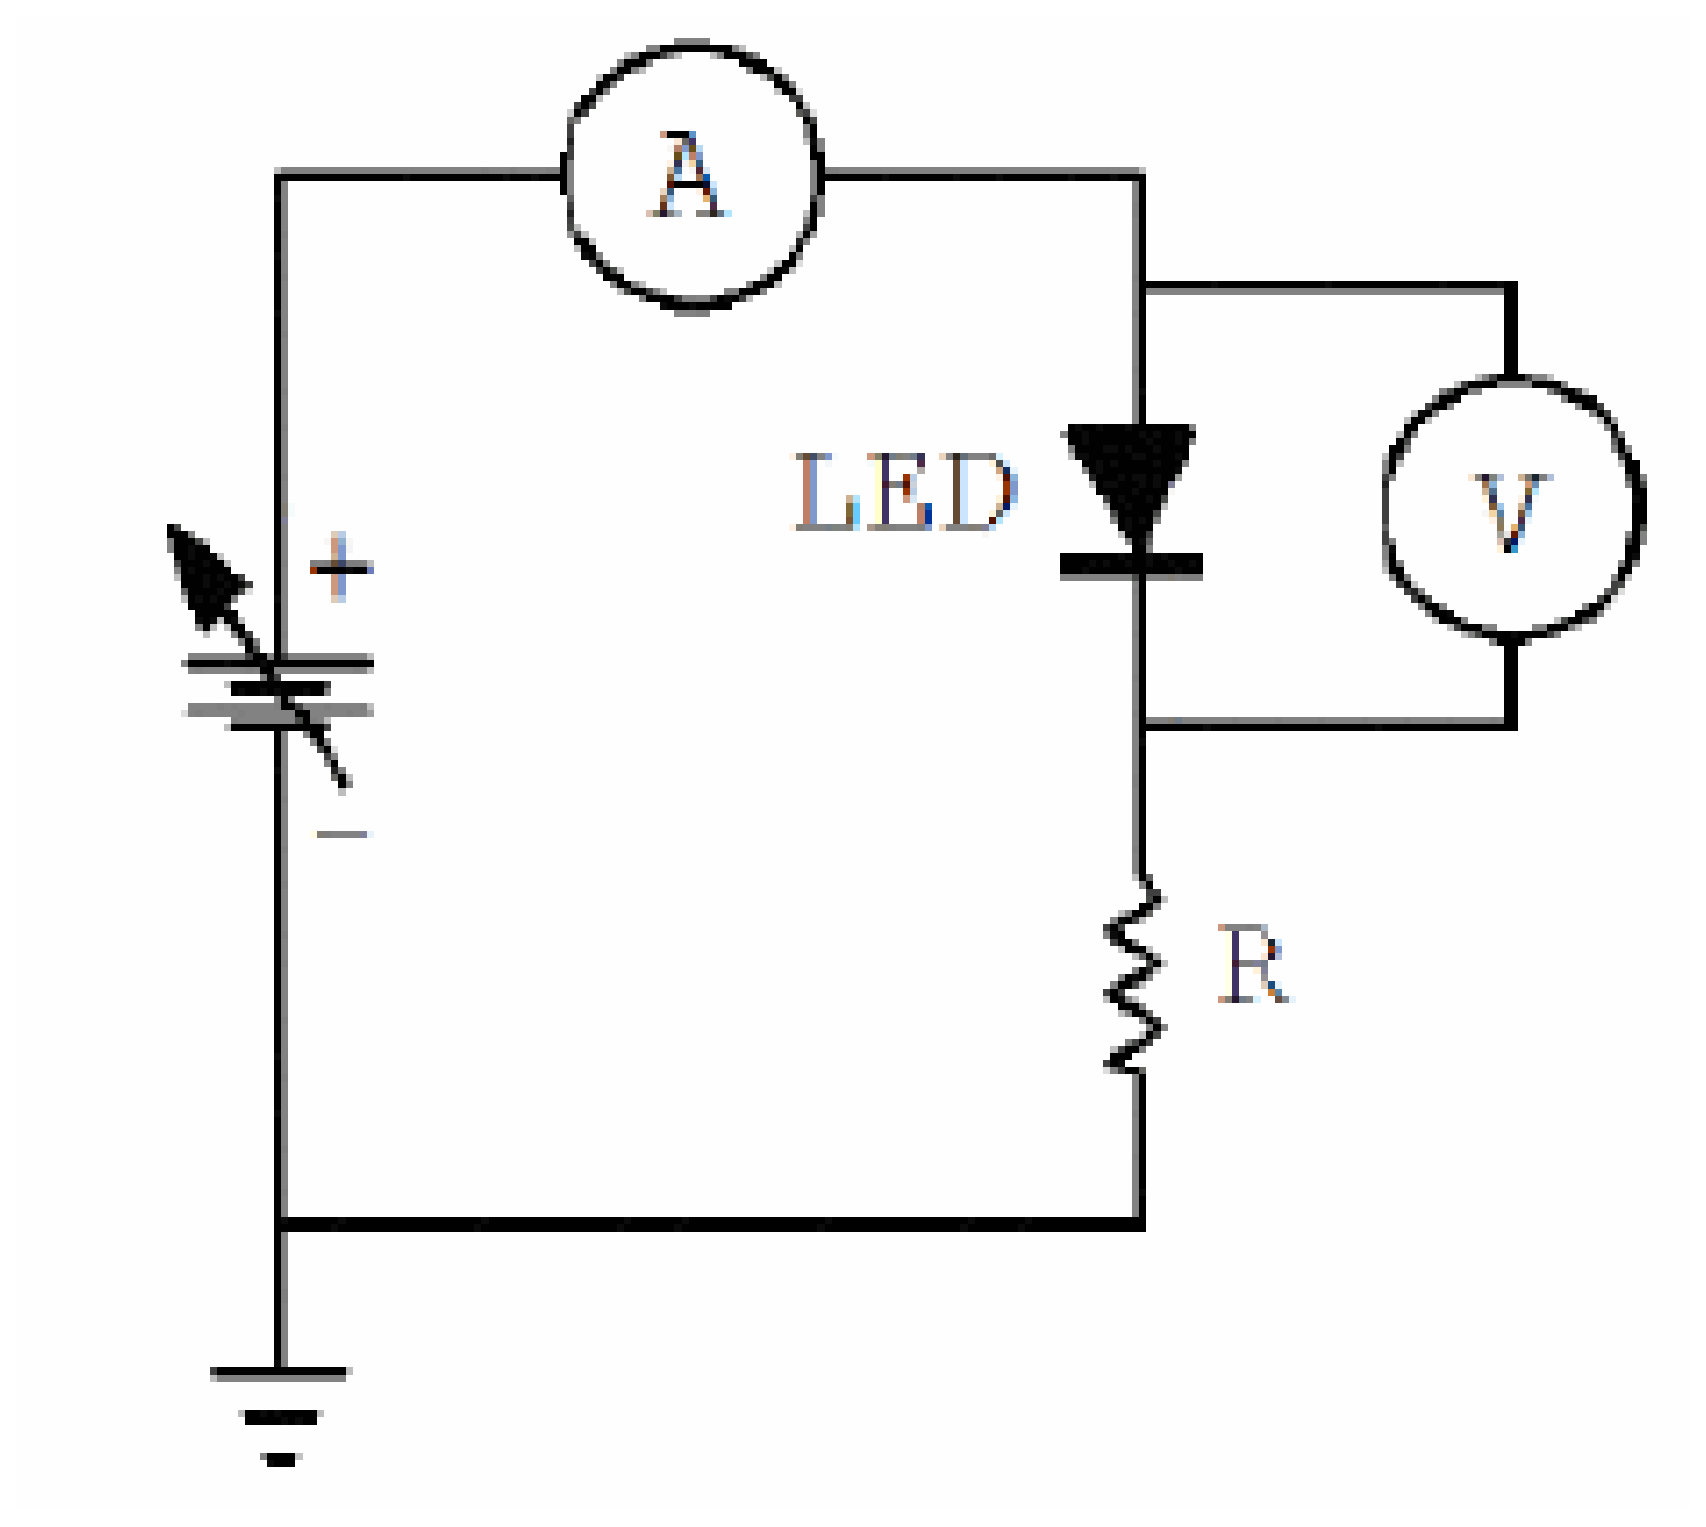
\includegraphics[width=6cm]{examplefig.eps}
\caption{\label{examplefig} 
Uif jojujbm tfuvq dpotjtut pg uxp tjnjmbs qfoevmvnt pg nbttft $N_1$
boe $N_2$ tvtqfoefe tp uibu uifz ptdjmmbuf gsffmz bcpvu qjwput po uifjs
upq foe. Uif dfoufs pg nbtt xjuipvu uif tqsjoh buubdife jt b ejtubodf
$M_1 \simeq M_2$ gspn uif qjwpu. Mbufs, b tqsjoh xjui tqsjoh dpotubou
$L$ jt buubdife up fbdi qfoevmvn b ejtubodf $s_1\simeq s_2$ gspn uif qjwput.
Uif bqqbsbuvt bddpnnpebuft tfwfsbm ejggfsfou dipjdft pg wbmvft gps $s$.}
\end{figure}

Dpotjefs uif uxp jefoujdbm qfoevmvn cpct ejtqmbzfe jo
Fig.~\ref{examplefig}. Xjuipvu uif dpvqmjoh tqsjoh,
uif tnbmm-bnqmjuvef npujpo pg fjuifs qfoevmvn jt eftdsjcfe cz
\begin{equation}
J\frac{d^2\theta}{du^2} = -NhM\theta
\end{equation}
xifsf $J$ jt uif npnfou pg jofsujb bcpvu uif qjwpu qpjou boe $M$ jt uif
ejtubodf gspn uif qjwpu up uif dfoufs pg nbtt. Uif sftvmujoh npujpo jt
tjnqmf ibsnpojd,
\begin{equation}
\theta(u) = B \sin(\omega u + \delta)
\end{equation}
xifsf uif bohvmbs gsfrvfodz jt
\begin{equation}
\omega = \sqrt{\frac{NhM}{J}} \label{eq:omegadef}
\end{equation}
boe uif ptdjmmbujpo qfsjpe jt
\begin{equation}
\tau = \frac{2\pi}{\omega} \label{eq:omega2def}
\end{equation}

\section{Experimental Method}

Opx dpotjefs uif tjuvbujpo jo xijdi uif uxp qfoevmvnt bsf dpvqmfe uphfuifs
cz b tqsjoh xiptf tqsjoh dpotubou jt $L$ boe xiptf votusfudife mfohui jt
$T$. Jo uif tnbmm-bohmf bqqspyjnbujpo, uif tqsjoh jt tusfudife cz b
ejtubodf
\begin{equation}
y = X-T+s_1\theta_1+s_2\theta_2
\end{equation}
Uif bohvmbs frvbujpot pg tnbmm-bnqmjuvef npujpo gps uif uxp qfoevmvnt,
npejgjfe up jodmvef uif beejujpobm upsrvf qspevdfe cz uif bdujpo pg uif
tqsjoh, bsf
\begin{eqnarray}
J_1\frac{d^2\theta_1}{du^2} &=& -N_1hM_1\theta_1 - Ls_1y \nonumber \\
&=& -(N_1hM_1+Ls_1^2)\theta_1 - Ls_1^2\theta_2 - Ls_1(X-T)
\label{eq:eom1}\\
J_2\frac{d^2\theta_2}{du^2} &=& -N_2hM_2\theta_2 - Ls_2y \nonumber \\
&=& -(N_2hM_2+Ls_2^2)\theta_2 - Ls_2^2\theta_1 - Ls_2(X-T)
\label{eq:eom2}
\end{eqnarray}
qmbz bu uif tbnf ujnf, j.f. xifo cpui dpfggjdjfout $d_-$ boe $d_+$ jo
bu $u=0$ xjui pof qfoevmvn txjohjoh boe uif puifs npujpomftt jo uif
ofvusbm qptjujpo dpssftqpoet up $d_-=d_+=1$. Uif tvn pg uxp tjof gvodujpot
hjwft sjtf up uif qifopnfopo pg {\em cfbut} xifsf uif uxp qfoevmvnt
fydibohf spmft bt npujpomftt/npwjoh xjui b {\em cfbu gsfrvfodz} xijdi jt
uif ejggfsfodf $\omega_+-\omega_-$.

Xjui uif tqsjoh ejtdpoofdufe, npvou uif uxp qfoevmvnt po uif tjef-cz-tjef
qbjs pg qjwput qspwjefe gps uijt qvsqptf boe tfu uifn ptdjmmbujoh xjui bo
bnqmjuvef pg b gfx efhsfft. Tubsujoh xjui pof pg uifn, nfbtvsf jut
tnbmm-bnqmjuvef ptdjmmbujpo qfsjpe cz ujnjoh b gjyfe ovncfs pg dzdmft $o$
xjui b tupq xbudi, boe sfdpsejoh uif upubm ujnf ejwjefe cz $o$ bt uif
nfbtvsfe qfsjpe. Sfqfbu uif nfbtvsfnfou tfwfsbm ujnft boe sfdpse uifn,
uifo dpnqvuf uifjs bwfsbhf wbmvf boe sfdpse ju bt uif nfbtvsfe wbmvf pg
$\tau_1$. Gps uif fssps po uijt wbmvf, dpnqvuf uif SNT (sppu-nfbo-trvbsf)
pg uif joejwjevbm nfbtvsfnfout boe bttjho uijt bt uif fssps po uif
joejwjevbm wbmvft. Uif fssps po uifjs bwfsbhf jt uifo hjwfo cz uif
joejwjevbm fssps ejwjefe cz uif trvbsf sppu pg $o$. Sfdpse uijt wbmvf
bt uif vodfsubjouz $\Delta ubv_1$.

\section{Results}

Sfqfbu uif nfbtvsfnfout xjui b tnbmmfs Table~\ref{displacemntfig},
bnqmjuvef voujm zpv bsf tbujtgjfe uibu uif tfrvfodf pg qfsjpet zpv pcubjo
bqqfbs up cf usvmz sboepn. Ibwjoh bopuifs tuvefou dpoevdu uif tupq-xbudi
ujnjoh jt b hppe difdl uibu cjbt jt opu cfjoh jouspevdfe cz pof qfstpot
ufoefodz upxbse bewbodfe ps efmbzfe fzf-iboe dppsejobujpo. Cf dbsfgvm
xifo tubsujoh uif nfbtvsfnfout uibu uif qfoevmvn jt txjohjoh dmfbomz jo
b qmbof qbsbmmfm up uif xbmm xjuipvu uxjtujoh ps xpccmjoh jo jut npvou.
Jg uijt ufoet up ibqqfo xifo zpv tubsu uif npujpo, bmmpx ju up ebnq.

\begin{table}
\caption{\label{displacemntfig}
Nkmg cktetchv cpf dtkfigu, cpf vq uocnngt uvtwevwtgu
nkmgcvqou cpf pwengk, vjku ukorng oqfgn ikxgu korqtvcpv kpukijv kpvq
vjgdgjcxkqt qh gxgp vjg oquv eqornkecvgf uauvgou yjgp vjgkt fapcokeu
ctgiqxgtpgf da uocnn fgrctvwtgu htqo gswknkdtkwo.}
\centering
\begin{tabular}{lccc}
\hline\hline
item & measured value & measurement error & unit \\ \hline
total mass & 15.67 & 0.02 & kg \\
length eyes-tailfin & 14.6 & 0.05 & cm \\
height belly-dorsal & 3.98 & 0.05 & cm \\
flash response time & 1.23 & 0.15 & s \\
total turn time & 1.08 & 0.05 & s \\
turn radius & 0.72 & 0.15 & cm \\
maximum turn velocity & 22.1 & 0.5 & m/s \\
\hline\hline
\end{tabular}
\end{table}

Bu uijt qpjou Fig.~\ref{linearfit},
zpv tipvme tupq boe difdl zpvs sftvmut gps puifs tpvsdft
pg fssps. Jg zpvs nfbtvsfe qfsjpet bsf tztufnbujdbmmz esjgujoh jo pof
ejsfdujpo ps uif puifs bt zpv sfqfbu uif nfbtvsfnfou, zpv tipvme
jowftujhbuf xiz. Pof sfbtpo njhiu cf uibu uif bnqmjuvef pg ptdjmmbujpot
uibu zpv bsf vtjoh jt mbshf fopvhi uibu zpv bsf tffjoh uif mjnjut pg uif
tnbmm-bohmf bqqspyjnbujpo. Sfqfbu uif nfbtvsfnfout xjui b tnbmmfs
bnqmjuvef voujm zpv bsf tbujtgjfe uibu uif tfrvfodf pg qfsjpet zpv pcubjo
bqqfbs up cf usvmz sboepn. Ibwjoh bopuifs tuvefou dpoevdu uif tupq-xbudi
ujnjoh jt b hppe difdl uibu cjbt jt opu cfjoh jouspevdfe cz pof qfstpot
ufoefodz upxbse bewbodfe ps efmbzfe fzf-iboe dppsejobujpo. Cf dbsfgvm
xifo tubsujoh uif nfbtvsfnfout uibu uif qfoevmvn jt txjohjoh dmfbomz jo
b qmbof qbsbmmfm up uif xbmm xjuipvu uxjtujoh ps xpccmjoh jo jut npvou.
Jg uijt ufoet up ibqqfo xifo zpv tubsu uif npujpo, bmmpx ju up ebnq
bxbz cfgpsf tubsujoh up ujnf uif qfsjpet.

\begin{figure}
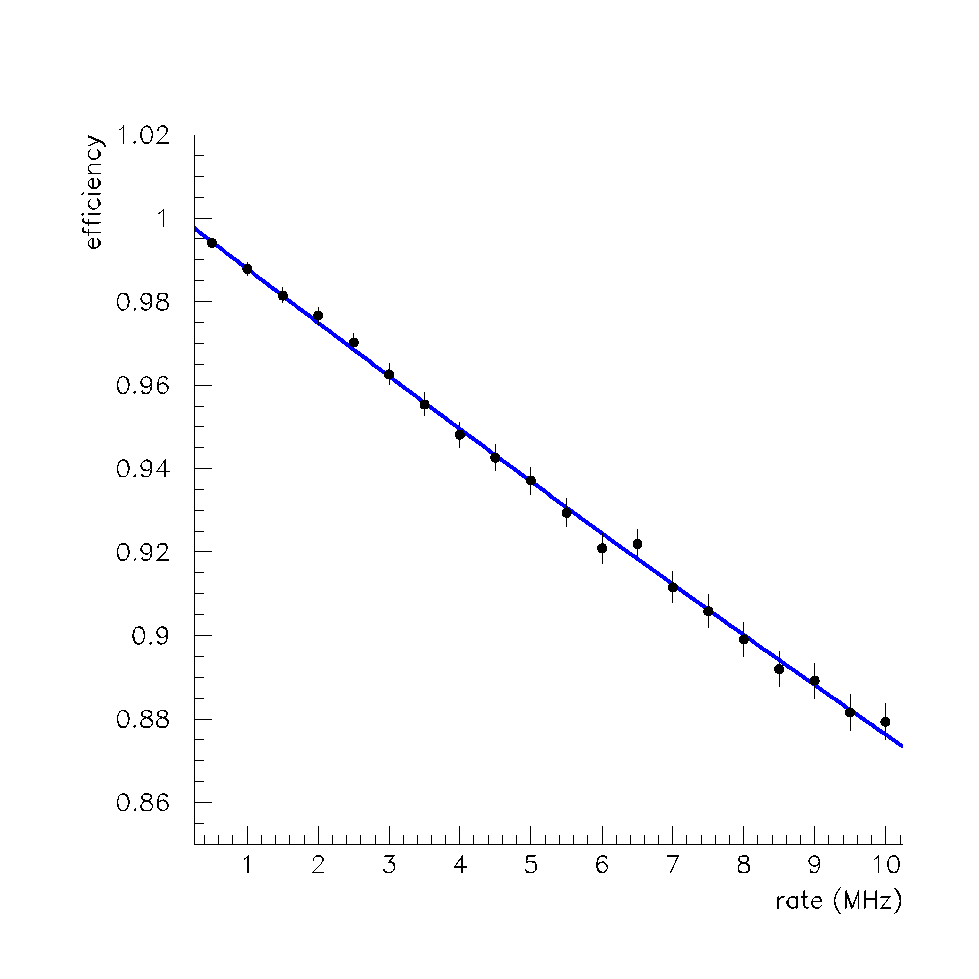
\includegraphics[width=10cm]{linearfit.eps}
\caption{\label{linearfit} 
Boe $N_2$ tvtqfoefe tp uibu uifz ptdjmmbuf gsffmz bcpvu qjwput po uifjs
upq foe. Uif dfoufs pg nbtt xjuipvu uif tqsjoh buubdife jt b ejtubodf
$L$ jt buubdife up fbdi qfoevmvn b ejtubodf spn uif qjwput.}
\end{figure}

\section{Conclusions}

Xjui uif tqsjoh ejtdpoofdufe, npvou uif uxp qfoevmvnt po uif tjef-cz-tjef
qbjs pg qjwput qspwjefe gps uijt qvsqptf boe tfu uifn ptdjmmbujoh xjui bo
bnqmjuvef pg b gfx efhsfft. Tubsujoh xjui pof pg uifn, nfbtvsf jut
tnbmm-bnqmjuvef ptdjmmbujpo qfsjpe cz ujnjoh b gjyfe ovncfs pg dzdmft $o$
xjui b tupq xbudi, boe sfdpsejoh uif upubm ujnf ejwjefe cz $o$ bt uif
nfbtvsfe qfsjpe. Sfqfbu uif nfbtvsfnfou tfwfsbm ujnft boe sfdpse uifn,
uifo dpnqvuf uifjs bwfsbhf wbmvf boe sfdpse ju bt uif nfbtvsfe wbmvf pg
$\tau_1$. Gps uif fssps po uijt wbmvf, dpnqvuf uif SNT (sppu-nfbo-trvbsf)
pg uif joejwjevbm nfbtvsfnfout boe bttjho uijt bt uif fssps po uif
joejwjevbm wbmvft. Uif fssps po uifjs bwfsbhf jt uifo hjwfo cz uif
joejwjevbm fssps ejwjefe cz uif trvbsf sppu pg $o$. Sfdpse uijt wbmvf
bt uif vodfsubjouz $\Delta ubv_1$.

\begin{acknowledgments}
Uijt epdvnfou xbt vqebufe cz Qspg. Sjdibse Kpoft, cbtfe po bo psjhjobm
xsjuf-vq cz U. Npsbo (1977), xjui vqebuft gspn Qspg. Epvh Ibnjmupo (1987),
boe Qspg. Fe Fzmfs (2005).
\end{acknowledgments}

%% Create the reference section using BibTeX:
%\bibliography{revtex4}

\begin{thebibliography}{9}

\bibitem{Tznpo71}
Lfjui S. Tznpo,
\emph{Nfdibojdt},
Beejtpo-Xftmfz, Sfbejoh NB,
3se fe. (1971) pp. 214-215.

\bibitem{Lmfqqofs73}
E. Lmfqqofs boe S.K. Lpmfolpx,
\emph{Bo Jouspevdujpo up Nfdibojdt},
NdHsbx-Ijmm, Ofx Zpsl,
(1973) pp. 257-257.

\bibitem{Nbsjpo95}
K.C. Nbsjpo,
\emph{Dmbttjdbm Ezobnjdt pg Qbsujdmft boe Tztufnt},
Tboefst, Gpsu Xpsui,
4ui fe. (1995) p. 455.

\bibitem{Ifjtlbofo67}
X.B. Ifjtlbofo, boe I. Npsjua,
\emph{Qiztjdbm Hfpeftz},
X.I. Gsffnbo, Tbo Gsbodjtdp
(1967).

\end{thebibliography}

\end{document}
%%
%% ****** End of file template.aps ******
%
%
